\documentclass[10pt]{article}
%Paketai----------------------------------------------
 \usepackage[L7x]{fontenc}
 \usepackage[lithuanian]{babel}
 \usepackage[utf8x]{inputenc}
 \usepackage{graphicx}
 %for eps
 %\usepackage{epstopdf}
 %%%%%%%%%%%%%%%%%%%%%%%%%%%%%%%
 \usepackage{latexsym}
 \usepackage{amssymb}
 \usepackage{amsmath}
 \usepackage{epsfig}
 \newtheorem{thm}{Teorema}
 \newtheorem{cor}[thm]{Išvada}
 \newtheorem{lem}[thm]{Lema}
 \newtheorem{prop}[thm]{Teiginys}
 \newtheorem{defn}[thm]{Apibrėžimas}
 \newtheorem{rem}[thm]{Pastaba}
 \def\institution#1{{\raggedright #1}}
 \def\address#1{\newline ${\ }$ \emph{#1}}
 \def\emaill#1{{\raggedright el.~paštas:\ {#1}}}
 \def\email#1{\newline {\raggedright ${\qquad\qquad}${#1}}}
 \def\dedication#1{\vspace{2mm}{\raggedright\qquad\emph{Dedikuotas {#1}}\vspace{2mm}}}
 \def\abstract#1{\vspace{2mm}{\raggedright\textbf{Santrauka}. {#1}\vspace{1mm}}}
 \def\keywords#1{{\raggedright\emph{Raktiniai žodžiai}: {#1}}}
 \def\Summary#1#2#3#4{\vspace{2mm}{\textbf{Summary}}\vspace{2mm}\newline{\textbf{#1}}\newline{\emph{#2}}\newline{#3}\newline{{\emph{Keywords:\ }}#4}}
 \def\boldhline{\noalign{\global\arrayrulewidth.8pt}\hline\noalign{\global\arrayrulewidth.4pt}}
% papildomi Paketai----------------------------------------------
 \usepackage{color}
\title{Kai kurie polivalentinių sistemų modeliavimo  aspektai}

\author{Irus Grinis${}^{1}$, Feliksas Ivanauskas${}^{1}$, Gediminas Stepanauskas${}^{1}$}
\date{ }
%literatūros sąrašas======================================================

%Literatūra
%
%
%
%[1] J. Mathai Mammen, Seok-Ki Choi, and George M. Whitesides. Polyvalent Interactions in Biological Systems: Implications for Design and Use of Multivalent Ligands and Inhibitors. Angewandte Chemie International Edition Volume 37, Issue 20:  2754–2794,  1998
%[2] Meyer B. Jackson. Molecular and Cellular Biophysics.  Cambridge University Press, 2006
%[3] Chinlin Guo and Herbert Levine. A statistical mechanics model for receptor clustering, Journal of Biological Physics , 26: 219-234, 2000
%
%[4] Lange K.  Applied Probability. Springer-Verlag, New York, 2003
%
%[5] Benjamin T.Houseman, Milan Mrksich. Model Systems for Studying Polyvalent Carbohydrate
%Binding Interactions. Topics in Current Chemistry. 218: 1-44, 2002.
%
%[6] Klein P, Pawson T, Tyers M. Mathematical modeling suggests cooperative interactions between a disordered polyvalent ligand and a single receptor site. Curr Biol. 13(19):1669-78, 2003 

\begin{filecontents*}{x.bib}
@ARTICLE{Grinis12,
 author={I. Grinis and F. Ivanauskas and G. Stepanauskas},
 title={ Some geometric aspects of polyvalent systems modeling},
 journal={Proc. of the Lithuanian Mathematical Society, Ser. B}, 
 volume={53},
 number={1},
 year={2012},
 pages={62-67},
 note={%Note}
}

@ARTICLE{Fasting12,
 author={C. Fasting and C.A. Schalley and M. Weber and O. Seitz and S. Hecht and B. Koksch and J. Dernedde and C. Graf and E.W. Knapp and R. Haag},
 title={ Multivalenz als chemisches Organisations- und Wirkprinzip },
 journal={Angewandte Chemie}, 
 volume={124},
 number={42},
 year={2012},
 pages={10622–10650},
 note={%Note}
}

@ARTICLE{Mammen98,
 author={J. Mathai Mammen and Seok-Ki Choi and George M. Whitesides},
 title={ Polyvalent Interactions in Biological Systems: Implications for Design and Use of Multivalent Ligands and Inhibitors},
 journal={Angewandte Chemie International Edition}, 
 volume={37},
 number={20},
 year={1998},
 pages={2754-2794},
 note={%Note}
}

@ARTICLE{Chinlin2000,
 author={Chinlin Guo and Herbert Levine},
 title={A Statistical Mechanics Model for Receptor Clustering},
 journal={Journal of Biological Physics},
 volume={26},
 number={3},
 year={2000},
 pages={219-234},
 note={%Note}
}

@ARTICLE{Houseman02,
 author={Benjamin T.Houseman and Milan Mrksich},
 title={Model Systems for Studying Polyvalent Carbohydrate Binding Interactions},
 journal={Topics in Current Chemistry},
 volume={218},
 number={1},
 year={2002},
 pages={1-44},
 note={%Note}
}

@ARTICLE{Klein03,
 author={Klein P and Pawson T and Tyers M.},
 title={Mathematical modeling suggests cooperative interactions between a disordered polyvalent ligand and a single receptor site},
 journal={Curr Biol.}, 
 volume={13},
 number={19},
 year={2003},
 pages={1669-1678},
 note={%Note}
}

@BOOK{Lange03,
   author = {Lange K.},
   title = {Applied Probability},
   publisher={Springer-Verlag},
   year = 2003
}

@BOOK{Trian10,
   author = { De Loera J.A. and Rambau J. and Santos F.},
   title = {Triangulations. Structures for Algorithms and Application},
   publisher={Springer-Verlag},
   year = 2010
}
\end{filecontents*}


%======================================================

%%% --------------------------------------------------------
\begin{document}
\maketitle
\vspace{-0.5cm}
{\small



\institution{${}^{1}$Vilniaus Universitetas, Matematikos ir informatikos fakultetas}
\address{Naugarduko g. 24, LT-03225 Vilnius, Lietuva}

\vspace{2mm}
\emaill{irus.grinis@mif.vu.lt; feliksas.ivanauskas@mif.vu.lt;}
\email{gediminas.stepanauskas@mif.vu.lt}

%\dedication{}
}

\abstract{ Šiame darbe nagrinėjami kai kurie polivalentinių sistemų modeliavimo geometriniai aspektai: ligandų ir receptorių sąveikos plokštumoje ir erdvėje }

\keywords{ polivalentinės sąveikos, receptoriai, ligandai, polivalentinės sistemos, matematinis modeliavimas  }
% ----------------------------------------------------------

%\nocite{*}
\section*{Įvadas}
%Mažos biologinės dalelės (atskiros molekulės, baltymo, DNR,  viruso, bakterijos ar pan.) valentingumas –- atskirų tos pačios rūšies jungčių su kita dalele skaičius (žr., pavyzdžiui, \cite{Grinis12}, dėl terminologijos). Atskira  jungtis (toliau ją vadinsime tiesiog ryšiu)   tarp dalelių formuojama sąveikos tarp ligando ir receptoriaus pagalba. Sąveikos, kurių valentingumas didesnis už vienetą, vadinamos polivalentinėmis. Mes nagrinėjame kai kuriuos geometrinius  polivalentinių sąveikų modeliavimo aspektus. Valentingumas priklauso nuo daugelio fizikinių, cheminių, geometrinių sąveikaujančiųjų dalelių   savybių. Atskirų polivalentinų sistemų analizei skirta  nemažai dėmesio (\cite{Mammen98}, \cite{Chinlin2000}, \cite{Houseman02},\cite{Klein03}) Šiame darbe  mes pateikiame ligando ir receptoriaus, receptorių paviršiaus, ligandų  komplekso abstrakčius  matematinius modelius, kurie gali būti panaudojami  kai kurių polivalentinių sąveikų analizėje. Straipsnio pabaigoje pateikiame algoritmą, kuris gali būti panaudotas ryšio tarp judančio taškinio ligando ir receptorių paviršiaus susidarymo tikimybei įvertinti.

Šiame straipsnyje mes tęsiame (žr. \cite{Grinis12}) kai kurių polivalentinių sąveikų  aspektų tyrinėjimus. 
Polivalentinė sistema  sudaryta iš dviejų  tipo objektų, kurie vadinami receptorių ir ligandų kompleksais. 
Minėtoji sistema  vadinama homogenine, jeigu bet kuris ligandas potencialiai gali sąveikauti, t.y. sudaryti ryšį, su bet kuriuo receptoriumi, priešingu atveju ją vadina nehomogenine. Sudarytų ryšių skaičius vadinamas valentingumu.

Polivalentinės  sistemos analizuojamos  \cite{Mammen98}, \cite{Chinlin2000}, \cite{Houseman02},\cite{Klein03} darbuose. Pagrindinis šio straipsnio tikslas -- valentingumo įvertinimas kai kuriais polivalentinių sistemų atvejais.

\section{Apibrėžimai, matematiniai modeliai ir jų aprašai}

%Tarkime, kad turime dviejų rūšių sąveikaujančius daleles. Viena rūšis (pavyzdžiui, bakterija, organizmo ląstelė) turi savo paviršiuje ar jo dalyje tam tikrą skaičių aktyvių vietų, kurias  vadinsime receptoriais. Matematiškai galima susieti minėtą paviršių su tam tikru geometriniu paviršiumi, o atskirą receptorių --  su tašku tame paviršiuje. Ligandai  sąveikauja su receptoriais pagal taisyklę: vienas ligandas -- vienas receptorius.  Ligandų ir receptorių vietą erdvėje susiesime su taškų, kuriuos vadinsime ligando ar receptoriaus centrais, koordinatėmis. Šiame darbe mes postuluojame, kad jeigu atstumas tarp ligando ir receptoriaus centrų mažesnis, negu nurodytas vadinamasis sąveikos spindulys, tai tarp jų atsiranda ryšys. Ryšio centru vadinsime atitinkamo receptoriaus centro koordinates.

Tarkime, kad turime dviejų rūšių sąveikaujančius objektus. Viena rūšis (pavyzdžiui, biologinė ląstelė ar jų grupė, baltymo ar DNR molekulė, socialinių individų grupė ir t.t. ) turi savybę sudaryti ryšį su kitos rūšies objektais (pavyzdžiui, virusais, mažomis molekulėmis, kitais individais ar socialiniais reiškiniais). Pirmos rūšies objektus vadinsime receptoriais, kitos -- ligandais. Bendru atveju mes tarsime, kad turime turime $N_R$ receptorių ir $N_L$ ligandų, kurie sudaro atitinkamus kompleksus, kurie savo ruožtu priklauso tam tikrai metrinei erdvei $X$.   

Ligando ir receptoriaus sąveiką apibūdina atitinkama \textit{ryšio susidarymo tikimybė} $P_R$, kuri priklauso nuo atstumo tarp jų centrų. Paprasčiausiu atveju $P_R$ yra lygi  vienam, jeigu atstumas tarp ligando ir receptoriaus centrų yra mažesnis už tam tikrą sąveikos spindulį $R_s$, ir nuliui priešingu atveju. Pastarasis atvejis buvo nagrinėjamas mūsų praeitame darbe. 

Ligandų ir receptorių kompleksai apibūdinami metrinės erdvės $X$ tam tikrų rutulių baigtinėmis sąjungomis: kiekvienas ligandas ir receptorius priklauso kokiam ,,nuosavam`` vienam ir tik vienam rutuliui.

Tarkime, kad turime receptorių kompleksą, kurio $n_R$ receptorių sąveikauja su tam tikrais $n_L  = n_R$ ligandais iš ligandų komplekso. \textit{Sąveikos energija} vadinsime tolydžią funkciją $n_L+n_R$ kintamųjų funkciją $E_S : X^{n_L+n_R} \to \mathbb{R}$, kurią laikysime  tam tikra atitinkamų atstumų erdvėje $X$ kompozicija.

Mūsų modelyje laikysime, kad minėtos abiejų kompleksų  sąveikos tikimybė priklauso tik nuo  sąveikos energijos. 

 
   






%Šiame darbe  nagrinėjame atvejį, kai dalelė su receptoriais yra pakankamai didelė, kad  ją pačią  ar  jos dalį   galėtume aproksimuoti tam tikru paviršiumi, pavyzdžiui,  plokštuma, sfera, elipsoidu (žr. pav. ~\ref{fig:d1a}).  Kita dalelė – ligandų kompleksas –  aprėžta plokštuminė sritis, kurioje yra $ N $  ligandų. Ignoruodami daugybę fizikinių  reiškinių, nagrinėjame paprastą  sąveikos  modelį: 
%\begin{itemize}
%
%\item vienas ligandas ar receptorius gali sudaryti ryšį atitinkamai tik su vienu receptoriumi ar ligandu;
%
%\item   ligandų kompleksas juda tiesiu keliu taip, kad jo trajektorija arba kerta receptorių dalelės paviršių, arba yra pakankamai arti jos, kad būtų prasminga skaičiuoti  ryšio tarp abiejų dalelių susidarymo tikimybę;
%
%\item iš visų $N$ ligandų pirmas suformuoja ryšį tas, kurio atstumas iki artimiausio receptoriaus yra  mažiausias ir neviršija sąveikos spindulio;
%
%\item  analogiškai antras ryšys atsiras tarp to ligando ir receptoriaus, tarp kurių atstumas mažiausias iš likusių ir t.t.  
%\end{itemize}
%               
%           
%Bendras susiformavusių pagal šią schemą ryšių skaičius  ir bus valentingumas. Modelis, kuris tenkina išvardintas savybes, vadinamas modeliu  be adaptacinės sąveikos. ~\ref{fig:dvivalentis}-e paveikslėlyje  iliustruojama dvivalenčio ligandų komplekso sąveika su receptoriais, kurios metu susiformuoja  abu ryšiai. Jeigu ligandų kompleksas po pirmo ryšio susiformavimo pradeda transformuotis tol, kol nebus galimybės susiformuoti dar vienam ryšiui, tai tokią sąveiką vadinama  adaptacine.  
%          

%\begin{figure}[h!]
%\centering {
%\begin{minipage}[t]{7.4cm}
%{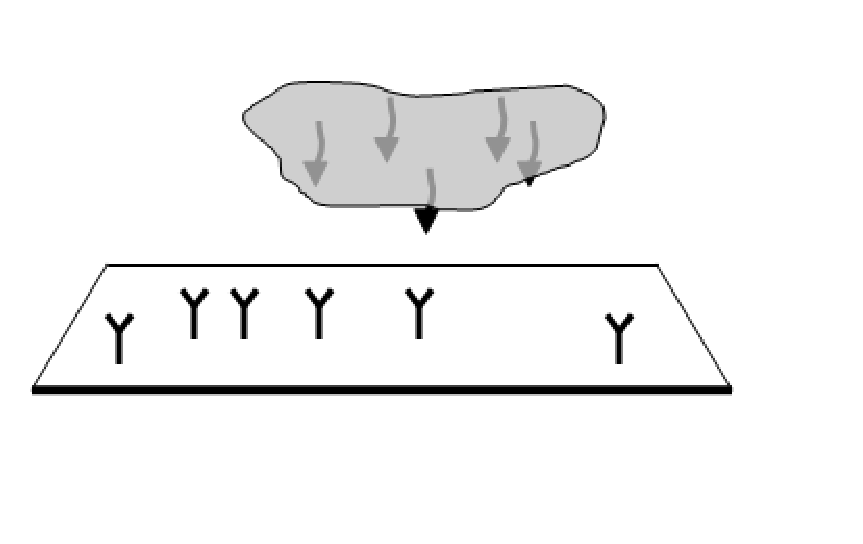
\includegraphics[ scale=0.5]{grinis1.eps}}
%\caption{Receptorių plokštuma ir ligandų kompleksas. }\label{fig:d1a}
%\end{minipage}
%}
%\end{figure}
%
%\begin{figure}[h!]
%\centering {
%\begin{minipage}[t]{7.4cm}
%{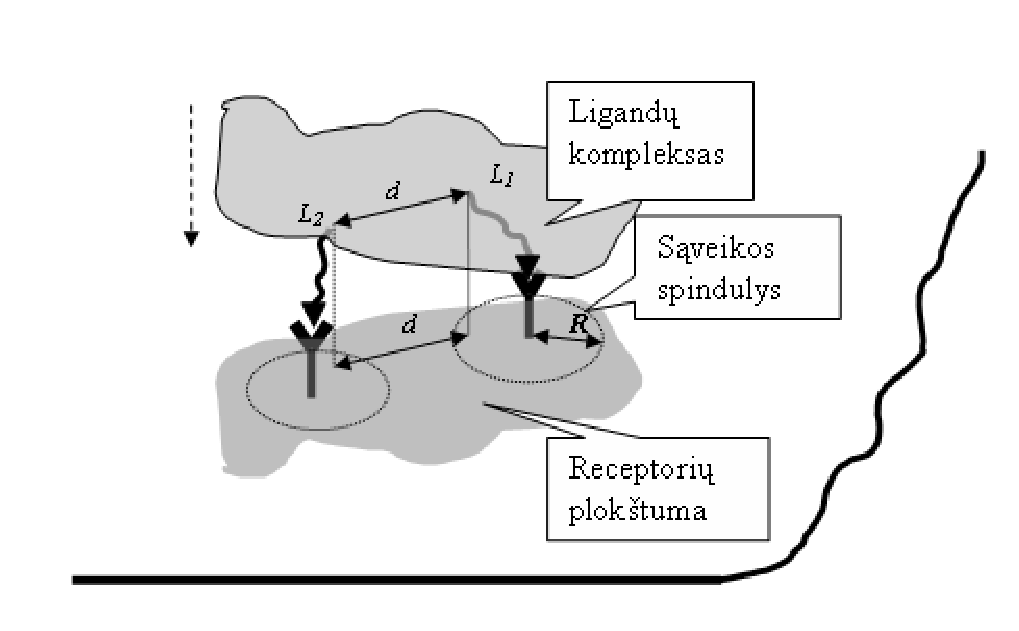
\includegraphics[ scale=0.5]{grinis2.eps}}
%\caption{Dvivalenčio ligandų komplekso ir receptorių plokštumos sąveika. Tam, kad susiformuotų abu ryšiai, reikia, kad abiejų ligandų centrai plokštumoje būtų nutolę nuo receptorių atstumu neviršijančiu $R$.}\label{fig:dvivalentis}
%\end{minipage}
%}
%\end{figure}

\section{Receptorių ir ligandų rutuliai}
%\subsection{Statusis kritimas}
%Tuo atveju, kai ligandų kompleksas labai mažas palyginus su 
%receptorių paviršiumi, galima tą paviršių modeliuoti plokštuma ar jos dalimi. 
%Pats paprasčiausias atvejis -- ligandų kompleksas, kurio visi ligandai yra vienoje plokštumoje, lygiagrečioje  receptorių plokštumai.Tarkime, kad ligandų kompleksas  krenta ant receptorių plokštumos 90 laipsnių kampu. Nagrinėsime ,,standartinį``  receptorių išsidėstymą plokštumoje, kai  jų centrai išsidėstę nepriklausomai vienas nuo kito pagal Puasono dėsnį (žr., pavyzdžiui, \cite{Lange03}) su intensyvumu $\lambda$:  tikimybė, kad spindulio $R$ skritulyje atsiras lygiai $k$ receptorių, yra $ \exp(-\lambda S_R)\frac{(\lambda S_R)^k}{k!} $, kur $S_R = \pi R^2$ -- minėto skritulio plotas. Visas sąveikas laikysime neadaptacinėmis. 


%----------------------------------------------------------  

%\begin{thm}\label{thm:1}
%Tegul receptorių centrai išsidėstę plokštumoje  pagal Puasono dėsnį su intensyvumu $\lambda$, o sąveikos spindulys yra $R$. Tada teisingi teiginiai:
%\begin{enumerate}
%	\item tikimybė, kad vienvalentinis ligando kompleksas susiformuos ryšį su kokiu nors receptoriumi plokštumoje, yra $1-\exp(-\lambda \pi R^{2})$;
%	\item jeigu $N$ ligandų kompleksas yra toks, kad tarp bet kokių dviejų ligandų atstumas  yra didesnis už $2R$, tai, tikimybė, kad susiformuos  visi $N$ ryšiai,  yra $(1-\exp(-\lambda \pi R^{2}))^N$;
%	\item ankstesnio punkto  sąlygomis  tikimybė, kad kompleksas  sudarys bent vieną ryšį, yra 
%	$1-\exp(-N \lambda \pi R^{2}))$;
%	\item antro punkto sąlygomis tikimybė, kad kompleksas susiformuos lygiai $k$ ryšių, yra 
%	 $ \binom{N}{k} \left( 1-\exp(-\lambda \pi R^{2}) \right) ^ k \exp(-(N-k) \lambda \pi R^{2})  $. 
%	
%	
%\end{enumerate}
%\end{thm}
%\textbf{Įrodymas}. 
%\begin{enumerate}
%\item  Minėtoji tikimybė lygi tikimybei, kad atsitiktinai paimtame plokštumos   R spindulio skritulyje atsiras bent vienas receptorius.
%\item Kadangi receptoriai išsidėstę nepriklausomai vienas nuo kito, tai tikimybė, kad  visuose $N$ nepersidengiančiuose skrituliuose atsiras bent po vieną receptorių, yra nepriklausomų įvykių tikimybių sandauga.
%\item Kadangi atstumas tarp ligandų yra didesnis už $2R$, tai atitinkami skrituliai, kuriuose turime rasti bent vieną receptorių sudarys bendrą plotą $\pi R^2 N $. Iš čia nesunkiai gauname reikiamą tikimybę.
%\item Yra  $\binom {N}{k}$ galimybių pasirinkti $k$ ligandų iš $N$ galimų,  kurių kiekvienas su tikimybe $\left( 1-\exp(-\lambda \pi R^{2}) \right) ^ k$ gali suformuoti ryšį, o likę $ N - k $ -- su tikimybe $\exp(-(N-k) \lambda \pi R^{2})$ -- jo nesuformuoti. 
%\end{enumerate}


%\subsection{Tiesiškai judančio taškinio ligando atvejai}
%Tarkime, kad turime vienvalentinį taškinį ligandą, kuris juda tiesiai, o jo trajektorija arba yra lygiagreti receptorių plokštumai, arba kerta ją tam tikrame taške.
%
%\subsubsection{Lygiagrečios trajektorijos atvejis}
%
%\begin{thm}\label{thm:2}
%Tegul receptorių centrai išsidėstę plokštumoje  pagal Puasono dėsnį su intensyvumu $\lambda$,  sąveikos spindulys yra $R$, o judančio taškinio ligando trajektorija yra lygiagreti plokštumai tiesė su atstumu iki jos  $ h $. Tada bet kurioje trajektorijos atkarpoje AB tikimybė, kad ligandas nesudarys ryšio su kokiu nors receptoriumi plokštumoje, yra $ \exp( -\lambda S(A,B)) $, čia 
%
%\[
%S(A,B) =
%\begin{cases}
%0, & \text{jeigu } h>R, \\
%
%\pi(R^2-h^2) + 2 \cdot distance(A,B) \cdot \sqrt{R^2-h^2}, & 
% \text{jeigu }  h \leqslant R.
%
%\end{cases}
%\]
%
%\end{thm}
%
%\textbf{Įrodymas}. Tiesiog reikia pastebėti, kad potencialiosios srities plokštumoje, kur gali susidaryti ryšys, plotas yra $ S(A,B) $.
%
%
%
%\subsubsection{Nelygiagrečios trajektorijos atvejis}
%
%\begin{thm}\label{thm:3}
%Tegul receptorių centrai išsidėstę plokštumoje  pagal Puasono dėsnį su intensyvumu $\lambda$,  sąveikos spindulys yra $R$, o judančio taškinio ligando trajektorija yra  tiesė, kuri kerta receptorių plokštumą ir sudaro su ja kampą $\alpha, \mbox{ } 0 < \alpha < \pi/2 $. Tada  tikimybė, kad ligandas nesudarys ryšio su kokiu nors receptoriumi  iki susidūrimo su plokštuma, yra $ \exp( -\lambda S_{\alpha}) $, čia 
%
%\[
%S_{\alpha} = \frac{1}{2} \pi R^2 \left(1 + \frac{1}{\sin \alpha } \right).
%\]
%\end{thm}
%
%\textbf{Įrodymas}. Pažymėkime $ k = \cot \alpha $. Paimkime tą trajektorijos dalį, kurioje atstumas iki plokštumos neviršija sąveikos spindulio  $ R $. Nemažindami bendrumo šiuo atveju galime nagrinėti atkarpą $ AB $, kur taškas $ A $ turi koordinates $ (0,0,R) $, o $ B $ atitinkamai  $ (kR,0,0) $, t.y., trajektorija kerta $ Ox $ ašį. Atkarpą  $ AB $ galima parametrizuoti taip:
%
%\[
%\begin{cases}
%x(t) = kRt, \\
%y(y) = 0, \\
%z(t) = R(1-t)
%\end{cases}
%\]
%čia $ t \in [0,1] $. Potencialioji sritis $ S_{\alpha} $, kurioje gali susidaryti ryšys, yra plokštumos $ Oxy $ skritulių , kurių centrai yra $ (x(t),0,0)$, o spinduliai $ R(t):=\sqrt{R^2-z^2(t)}=R\sqrt{(2-t)t} $, sąjunga.
%Nesunku matyti, kad, kai $ t $ keičiasi nuo $ 0 $ iki tam tikro $ t_0 $, minėti skrituliai ,,auga`` taip, kad yra vienas į kitą įdėti. 
%Iš tikrųjų, kai $ R(0)=0 $,  turime vieną tašką. Kai $ t \in \left( 0,1 \right)\mbox{, turime } R'(t) \geq 0 \mbox{ ir tik } R'(1)=0 $. Iš kitos pusės, minėtų skritulių ,,kairiausias`` taškas $ x_{min}(t) := x(t) - R(t) = R(kt-\sqrt{(2-t)t}) $ pasižymi tuo, kad $ x_{min}'(t) < 0 $, kai $ t \in [0, t_{0}) $, čia 
%$ t_{0} = 1 - \frac{k}{\sqrt{k^2+1}} = 1 - \cos \alpha  $.
%
%Kai $ t \in [t_{0}, 1] $ panagrinėkime aukščiau minėtų skritulių, tiksliau juos ribojančių apskritimų, gaubtinę. Bendroji apskritimų lygtis yra
%$$ (x-x(t))^2 + (y-y(t))^2 - R^2(t) = 0, $$ 
%t.y.,
%$$ (x-Rkt)^2 + y^2 - R^2t(2-t) = 0 . $$ 
%Diferencijuodami pagal $ t $, turime 
%$$ kx-k^2Rt+R-Rt = 0,  $$
%t.y.,
%$$
%	t=\frac{kx+R}{R(1+k^2)}
%$$
%Įstatę $ t $ į apskritimų lygtį, gauname  gaubtinės -- elipsės lygtį:
%
%\[\frac{{R}^{2}+2kxR+\left( -{k}^{2}-1\right) \,{y}^{2}-{x}^{2}}{{k}^{2}+1}=0, \]
%kurią galima užrašyti taip:
%\[\frac{{\left( x-kR\right) }^{2}}{\left( {k}^{2}+1\right) \,{R}^{2}}+\frac{{y}^{2}}{{R}^{2}}=1.\]
%
%
%Dabar nesunkiai gauname srities $ S_{\alpha} $ plotą. Reikia paimti pusę minėtos elipsės ploto ir pridėti dar  pusę spindulio $ R $ skritulio ploto (žr. ~\ref{fig:teoremai3} pav.). 
%
%
%
%\begin{figure}[h!]
%\centering {
%\begin{minipage}[t]{7.4cm}
%{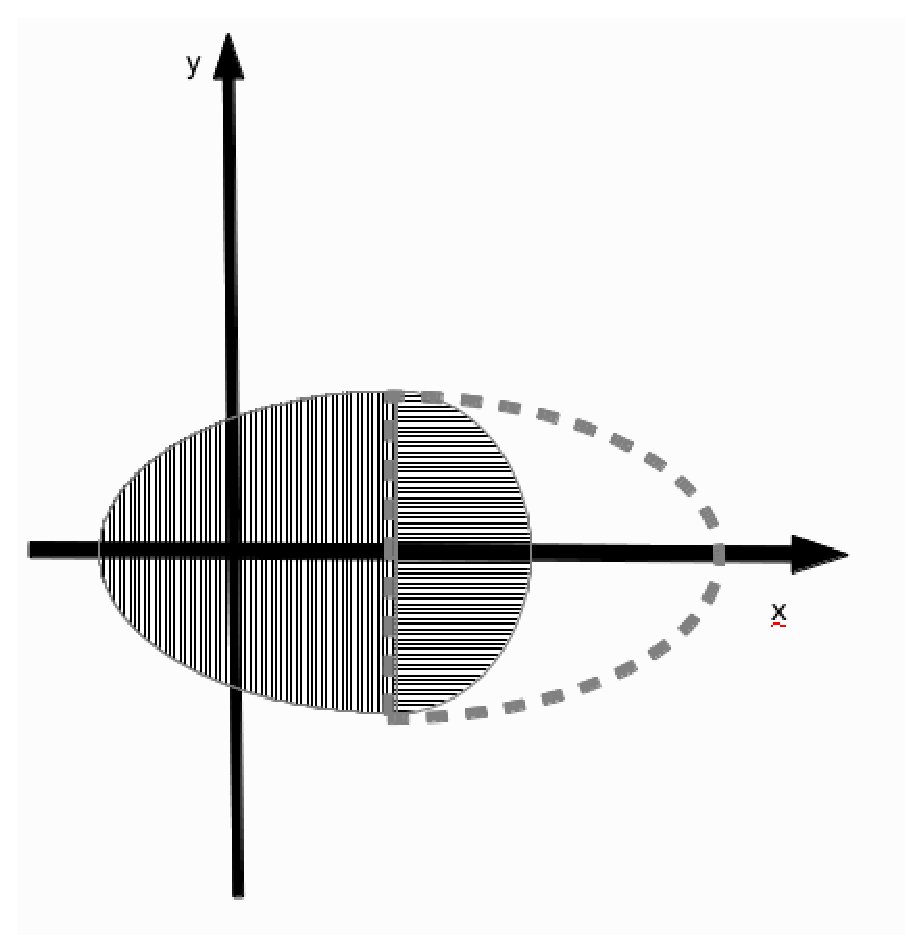
\includegraphics[ scale=0.45]{grinis3.eps}}
%\caption{Brėžinys teoremai 3. Sritis $ S_{\alpha} $ sudaryta iš dviejų dalių: pusės elipsės ir pusės skritulio.}\label{fig:teoremai3}
%\end{minipage}
%}
%\end{figure}




\section{Ryšių skaičiaus įvertinimo algoritmas: Puasono modelis}

%Šiame skyriuje panagrinėsime receptorių ir ligandų sąveiką trimatėje erdvėje. Tarkime, kad dalelė su receptoriais yra uždaras iškilus  glodus (klasės $ C^1 $) paviršius, kurio vidų žymėsime $ B $, o $ \delta B  $ -- patį paviršių. Reikalausime papildomai, kad bet kuri  spindulio $R$ sfera, kurios centras guli viduje $ B $ ir yra nutolęs nuo  paviršiaus daugiau negu $ R $, pilnai priklausytų sričiai $ B $.  Vėl tarsime, kad receptoriai išsidėstę paviršiuje  pagal Puasono dėsnį su parametru $ \lambda $.
%
%Pavyzdys. Nurodyto paviršiaus pavyzdys -- elipsoidas, kurio visos ašys yra didesnės už $ 2R $.


 
%\subsection{Skaitinis ryšio susidarymo tikimybės skaičiavimo algoritmas}
%Tarkime, kad paviršius $ \delta B $ duotas neišreikštine formule $ F(x,y,z) = 0 $. Judančio vienvalenčio taškinio ligando trajektorija tegul būna tiesės atkarpa $ T_{1}T_{2} $, kurios galai žinomi iš anksto. Galime naudoti tokį  algoritmą ryšio susidarymo tikimybei rasti.
%
%\begin{enumerate}
%\item Sudarome paviršių $ \delta B $ aproksimuojantį tinklelį. Vienas iš būdų sukurti paviršiaus tinklelį -- pasinaudoti kokiu nors trianguliacijos algoritmu (dėl apibrėžimų žr., pavyzdžiui, \cite{Trian10}  ). Panaudodami  paviršiaus $ \delta B $ savybes, konstruojame jos $ B $ aproksimaciją daugiasieniu, tenkinančiu savybes:
%\begin{itemize}
%
%\item kiekviena daugiasienio viršūnė priklauso $ \delta B $;
%
%\item kiekviena jo siena -- trikampis, kurio visi taškai nutolę nuo $ \delta B $ ne daugiau, negu nustatytas rėžis $ \epsilon $.
%
%\end{itemize}
%
%\item Tardami, kad ligandas juda nuo $ T_1 $, patikriname, ar jis kertą paviršių $ \delta B $. Jeigu taip -- perkeliame tašką $ T_2 $ į susikirtimo vietą.
%
%\item Pasirenkame aproksimuojančio daugiasienio sienas, kurių taškai nutolę nuo atkarpos $ T_{1}T_{2} $ ne daugiau, negu per sąveikos spindulį $ R $. Tam galima panaudoti anksčiau pateiktas teoremas 2 ir 3, nes užtenka patikrinti ar atitinkama siena, t.y., trikampis, kertasi su atitinkama sritimi, kur gali susidaryti ryšys,  to trikampio  plokštumoje ir apskaičiuoti sankirtos plotą.
%
%\item Sumuojame visus praeitame žingsnyje minėtus sankirtų plotus.
%
%\item Apskaičiuojame ryšio atsiradimo tikimybę.
%   
%\end{enumerate}



%Šitą algoritmą galima pritaikyti įvairiems tikslams. Vienas iš jų -- Monte Carlo simuliacijos. Pavyzdžiui, galima generuoti ,,atsitiktines`` atkarpas ir skaičiuoti ryšio susidarymo tikimybę kiekvienai iš jų, o po to įvertinti bendrą ryšio susidarymo tikimybę ,,atsitiktinai judantiems`` ligandams.


\bibliographystyle{plain}
\bibliography{x}
\Summary{Some geometric aspects of polyvalent systems modeling }{I.Grinis, F. Ivanauskas and G.Stepanauskas}{ In this paper we consider the interaction of ligands and receptors on the plane and in the  space}{ polyvalent interactions, receptors, ligands, polyvalent systems, mathematical modeling}
\end{document}

